\documentclass{article}%
\usepackage[T1]{fontenc}%
\usepackage[utf8]{inputenc}%
\usepackage{lmodern}%
\usepackage{textcomp}%
\usepackage{lastpage}%
\usepackage[head=40pt,margin=0.5in,bottom=0.6in]{geometry}%
\usepackage{graphicx}%
%
\title{\textbf{Comunidades de Palevecino en Lara protestan por falta de gas}}%
\author{El Nacional Web}%
\date{15/11/2018}%
%
\begin{document}%
\normalsize%
\maketitle%
\textbf{URL: }%
http://www.el{-}nacional.com/noticias/protestas/comunidades{-}palevecino{-}lara{-}protestan{-}por{-}falta{-}gas\_259839\newline%
%
\textbf{Periodico: }%
EN, %
ID: %
259839, %
Seccion: %
Protestas\newline%
%
\textbf{Palabras Claves: }%
Lara, Protestas, Gobierno\newline%
%
\textbf{Derecho: }%
2.8%
, Otros Derechos: %
NO\_TIENE%
, Sub Derechos: %
2.8.1%
\newline%
%
\textbf{EP: }%
SI\newline%
\newline%
%
\textbf{\textit{Los manifestantes están a la altura del sector La Mendera}}%
\newline%
\newline%
%
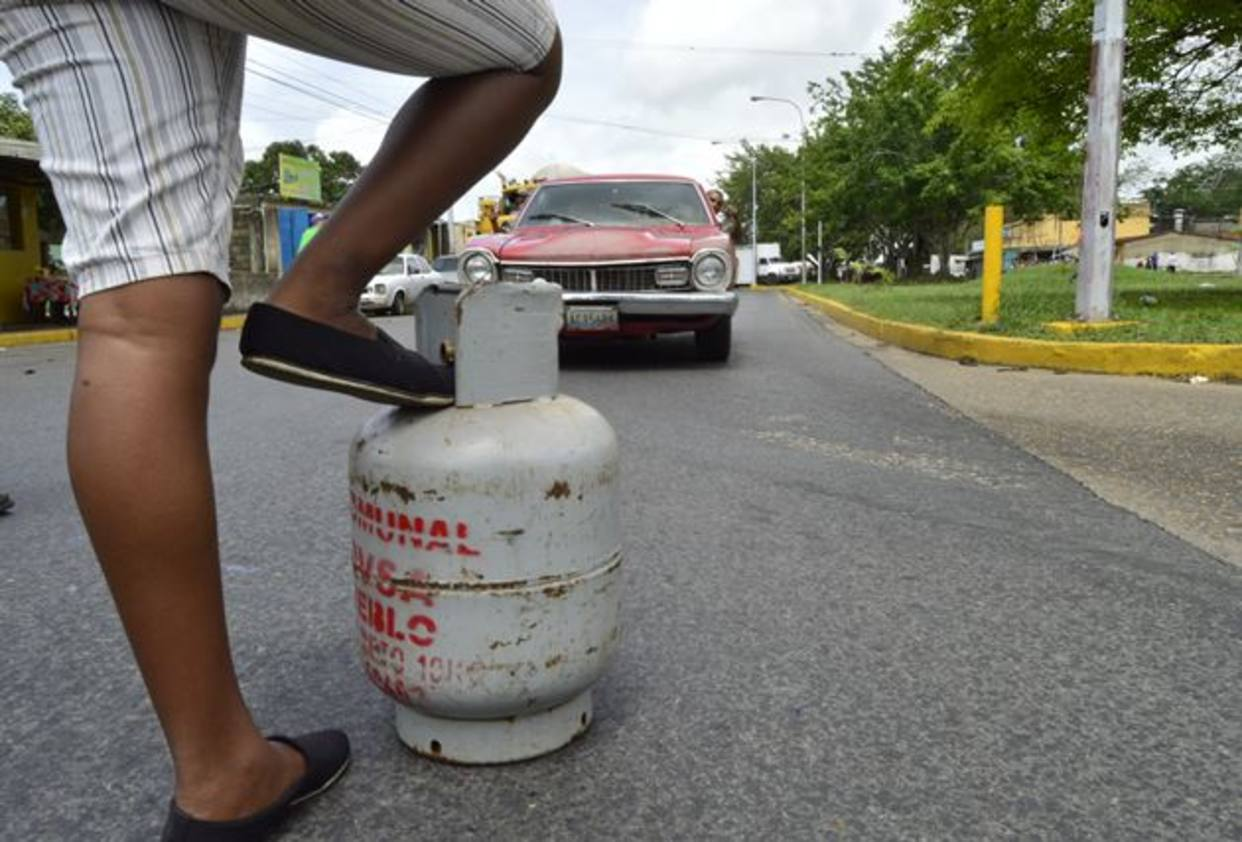
\includegraphics[width=300px]{34.jpg}%
\newline%
%
Habitantes de varias comunidades del municipio Palavecino, estado Lara, protestan este jueves en la avenida Ribereña por falta de distribución de~gas.%
\newline%
%
Reportes de Twitter indican que los manifestantes están a la altura del sector La~Mendera y que la avenida Libertador de Cabudare permanece trancada.%
\newline%
%
En varias regiones del país se registran~protestas diarias por fallas en los servicios básicos de agua, electricidad, transporte, alimentos y~gas.%
\newline%
%
\end{document}